\documentclass[a4paper]{article}
\usepackage{import}
\usepackage[utf8]{inputenc}
\usepackage[T1]{fontenc}
\usepackage{textcomp}
\usepackage[italian]{babel}
\usepackage{amsmath, amssymb}
\usepackage{booktabs,xltabular}
\usepackage{amsfonts}
\usepackage{subcaption}
\usepackage{amsthm}
\usepackage{cancel}
\usepackage{mdframed}
\usepackage{makecell}
\usepackage{float}
\usepackage{xcolor}
\usepackage{listings}
\usepackage{gensymb}
\usepackage{graphicx}
\usepackage{bodeplot}
\usepackage{physics}
\usepackage{tikz}
\usetikzlibrary{shapes, arrows, automata, petri, decorations.markings, decorations.pathreplacing, positioning, calc, quotes}
\usepackage{circuitikz}
\usepackage[label=corner]{karnaugh-map}
\graphicspath{{./figures/}}

% Set default font to sans-serif
\renewcommand{\familydefault}{\sfdefault} 
\usepackage{eulervm}

\usepackage{forest}

\usepackage{mathtools}
\DeclarePairedDelimiter\ceil{\lceil}{\rceil}
\DeclarePairedDelimiter\floor{\lfloor}{\rfloor}

% \usepackage{ntheorem}

\usepackage{import}
\usepackage{pdfpages}
\usepackage{transparent}
\usepackage{xcolor}

\usepackage{hyperref}
\hypersetup{
    colorlinks=false,
}

% Code blocks
\definecolor{codegreen}{rgb}{0,0.6,0}
\definecolor{codegray}{rgb}{0.5,0.5,0.5}
\definecolor{codepurple}{rgb}{0.58,0,0.82}
\definecolor{backcolour}{rgb}{0.95,0.95,0.95}

\lstdefinestyle{mystyle}{
	backgroundcolor=\color{backcolour},
	commentstyle=\color{codegreen},
	keywordstyle=\color{magenta},
	numberstyle=\tiny\color{codegray},
	stringstyle=\color{codepurple},
	basicstyle=\ttfamily\footnotesize,
	breakatwhitespace=false,
	breaklines=true,
	captionpos=b,
	keepspaces=true,
	numbers=left,
	numbersep=5pt,
	showspaces=false,
	showstringspaces=false,
	showtabs=false,
	tabsize=2
}

\lstset{style=mystyle}

\usepackage{color}
\usepackage{import}
\usepackage{pdfpages}
\usepackage{transparent}
\usepackage{xcolor}

% Example frame
\theoremstyle{definition}
\newmdtheoremenv[%
	linecolor=gray,leftmargin=0,%
	rightmargin=0,
	innertopmargin=8pt,%
	innerbottommargin=8pt,
	ntheorem]{example}{Esempio}[section]

% Important definition frame
\theoremstyle{definition}
\newmdtheoremenv[%
	linecolor=gray,leftmargin=0,%
	rightmargin=0,
	backgroundcolor=gray!40,%
	innertopmargin=8pt,%
	innerbottommargin=8pt,
	ntheorem]{definition}{Definizione}[section]

% Exercise frame
\theoremstyle{definition}
\newmdtheoremenv[%
	linecolor=gray,leftmargin=0,%
	rightmargin=0,
	innertopmargin=8pt,%
	innerbottommargin=8pt,
	ntheorem]{exercise}{Esercizio}[section]

% Theorem frame
\theoremstyle{definition}
\newmdtheoremenv[%
  linecolor=gray,leftmargin=0,%
  rightmargin=0,
  innertopmargin=8pt,%
  innerbottommargin=8pt,
  ntheorem]{theorem}{Teorema}[section]

\theoremstyle{definition}
\newmdtheoremenv[%
  linecolor=white,leftmargin=0,%
  rightmargin=0,
  innertopmargin=8pt,%
  innerbottommargin=8pt,
  ntheorem]{define}{Definizione utile}[section]

% figure support
\usepackage{import}
\usepackage{xifthen}
\pdfminorversion=7
\usepackage{pdfpages}
\usepackage{transparent}
\newcommand{\incfig}[1]{%
	\def\svgwidth{\columnwidth}
	\import{./figures/}{#1.pdf_tex}
}

% FSM tikz
\tikzset{
    place/.style={
        circle,
        thick,
        draw=black,
        minimum size=6mm,
    },
        state/.style={
        circle,
        thick,
        draw=black,
        fill=white,
        minimum size=6mm,
    },
}

\pdfsuppresswarningpagegroup=1

\usepackage{pgfplots}
\pgfplotsset{compat=1.18,width=10cm}

% Save plots as pdf and reuse them without compiling every time
\usetikzlibrary{external}
\tikzexternalize[prefix=figures/tikz/, optimize=false]


\begin{document}

\begin{titlepage}
	\begin{center}
		\vspace*{1cm}

		\Huge
		\textbf{Probabilità e Statistica\\Esercizi}

		\vspace{0.5cm}
		\LARGE
		UniVR - Dipartimento di Informatica

		\vspace{1.5cm}

		\textbf{Fabio Irimie}

		\vfill


		\vspace{0.8cm}


		2° Semestre 2023/2024

	\end{center}
\end{titlepage}


\tableofcontents
\pagebreak

\section{Introduzione}
\subsection{Cos'è l'informatica?}
È una scienza che studia la calcolabilità, cioè cerca di capire che problemi si possono
risolvere con un programma. Nasce dall'unione di matematica, ingegneria e logica. Il
computer è solo uno strumento, mentre la matematica è il linguaggio con cui si
creano algoritmi che permettono di risolvere i problemi.

\subsection{Origini dell'informatica}
Hilbert, nel 1900, si pose l'obiettivo di formalizzare tutta la matematica con un insieme
finito e non contraddittorio di assiomi. Nel 1931, invece, Gödel dimostrò che l'informatica
non potrà mai rappresentare tutta la matematica, perché ci saranno sempre proposizioni
vere ma non dimostrabili tramite il calcolo. Ci si iniziò a chiedere se esistessero
modelli di calcolo meccanici in grado di risolvere tutti i problemi. Nel 1936, Turing
propose la macchina di Turing, una \textbf{sola} macchina programmabile in grado di
risolvere tutti i problemi risolvibili:
\[
  Int(P,x) = \begin{cases}
    P(x) & \text{se } P(x) \text{ termina}\\
    \uparrow & \text{se } P(x) \text{ non termina}
  \end{cases}
\] 
dove $P$ è un programma e $x$ è un input. La macchina di Turing è un modello teorico
di calcolatore, che non esiste fisicamente, ma è in grado di simulare qualsiasi altro
calcolatore. Da questo modello deriva la concezione di calcolabilità, cioè se un problema
è intuitivamente calcolabile, allora esiste un programma in grado di risolverlo.

Altri modelli di calcolo che sono stati proposti sono:
\begin{itemize}
  \item Lambda-calcolo
  \item Funzioni ricorsive
  \item Linguaggi di programmazione (Turing-completi)
\end{itemize}

\begin{define}
  La Turing-completezza è la proprietà di un linguaggio di programmazione di essere
  in grado di simulare una macchina di Turing, cioè di poter risolvere qualsiasi problema
  risolvibile.
\end{define}

\subsubsection{Calcolabilità}
Un programma è calcolabile se termina, ma non è detto che termini in un tempo ragionevole.
Non esistono algoritmi che possono dire se un programma termina o meno. Questo è un esempio
di problema non calcolabile.

I problemi non calcolabili sono infinitamente più numerosi di quelli calcolabili

\section{Funzioni calcolabili}
Un insieme è una proprietà ed è rappresentato da una funzione che indica se un elemento
appartiene o meno all'insieme. I problemi da risolvere (in questo corso) hanno come
soluzione una funzione sui naturali:
\[
  f : \mathbb{N} \to \mathbb{N}
\] 
Questo tupo di funzione è un \textbf{insieme} di associazioni input-output. Un esempio
è la funzione quadrato:
\[
  f = \text{quadrato} = \{(0,0), (1,1), (2,4), (3,9), \ldots\} = \{(n,n^2) | n \in \mathbb{N}\}
\] 
Quindi \( f \) è un insieme di coppie in \( \mathbb{N} \subseteq \mathbb{N} \times \mathbb{N} \) la
cui cardinalità è: \( \left| \mathbb{N} \times \mathbb{N} \right| =
\left| \mathbb{N} \right| \). Di conseguenza la funzione è un sottoinsieme di \( \mathbb{N}
\times \mathbb{N}\):
\[
  f \subseteq \mathbb{N} \times \mathbb{N} \quad f \in \mathcal{P}(\mathbb{N} \times \mathbb{N})
\] 
Dove \( \mathcal{P}(\mathbb{N} \times \mathbb{N}) \) è l'insieme delle parti di \( \mathbb{N}
\times \mathbb{N} \), cioè l'insieme di tutti i sottoinsiemi di \( \mathbb{N} \times
\mathbb{N} \).

Il numero di funzioni è:
\[
  f: \mathbb{N} \to \mathbb{N} = \left| \mathcal{P}(\mathbb{N} \times \mathbb{N}) \right| 
  = \left| \mathcal{P}(\mathbb{N}) \right| 
\] 
\begin{example}
  Un esempio di insieme delle parti per l'insieme \( A = \{1,2,3\} \) è:
  \[
    \mathcal{P}(A) = \{\emptyset, \{1\}, \{2\}, \{3\}, \{1,2\}, \{1,3\}, \{2,3\}, \{1,2,3\}\}
  \] 
  E le cardinalità sono:
  \[
    \left| A \right| = 3 \quad \left| \mathcal{P}(A) \right| = 8 = 2^3
  \] 
  \[
    \downarrow
  \] 
  \[
    \left| \mathbb{N} \right| = \omega < 
    \underbrace{\left| \mathcal{P}(\mathbb{N}) \right| = 2^{\omega}}_{%
      \substack{\text{Insieme delle funzioni,}\\ 
      \text{non numerabile}}
    }
    = \left| \mathbb{R} \right| 
  \] 
\end{example}
Si ha quindi che \textbf{l'insieme delle funzioni non è numerabile}

\vspace{1em}
\noindent
Ci si chiede se queste funzioni sono tutte calcolabili:
\begin{definition}
  Una funzione \textbf{intuitivamente calcolabile} è una funzione descrivibile attraverso
  un algoritmo, cioè una sequenza finita di passi discreti elementari.
\end{definition}

\subsection{Quante funzioni numerabili ci sono?}
Consideriamo \( \Sigma \) come un alfabeto finito, cioè una seguenza di simboli
utilizzabili per scrivere un programma o algoritmo.
\[
  \Sigma = \{s_1,s_2,s_3, \ldots, s_n\}
\] 
\[
  \downarrow
\] 
\[
  \text{Programma} \subseteq \text{sqeuenze di simboli in } \Sigma
\] 
Con \( \Sigma^* \) si descrive l'insieme di tutte le sequenze finite di simboli in \( \Sigma \),
quindi l'insieme di tutti i possibili programmi è:
\[
  \text{Programmi} \subseteq \Sigma^*
\]

\begin{example}
  Se \( \Sigma = \left\{ a, b, c \right\} \) allora la sequenza di tutti i possibili
  simboli è:
  \[
    \Sigma^* = \{\epsilon, a, b, c, aa, ab, ac, ba, bb, bc, ca, cb, cc, aaa, aab, \ldots\}
  \]
  dove \( \epsilon \) è la stringa vuota.

  La cardinalità di \( \Sigma^* \) è infinita numerabile (anche se \( \Sigma  \) è finito).
  \[
    \left| \Sigma^* \right| = \left| \mathbb{N} \right| 
  \] 
\end{example}

Si ha quindi che l'insieme dei programmi è numerabile:
\[
  \left| \text{Programmi in } \Sigma \right| \leq \left| \Sigma^* \right| = \left| \mathbb{N} \right|
\] 
e questo implica che l'insieme delle \textbf{funzioni calcolabili è numerabile}

\begin{figure}[H]
  \centering
  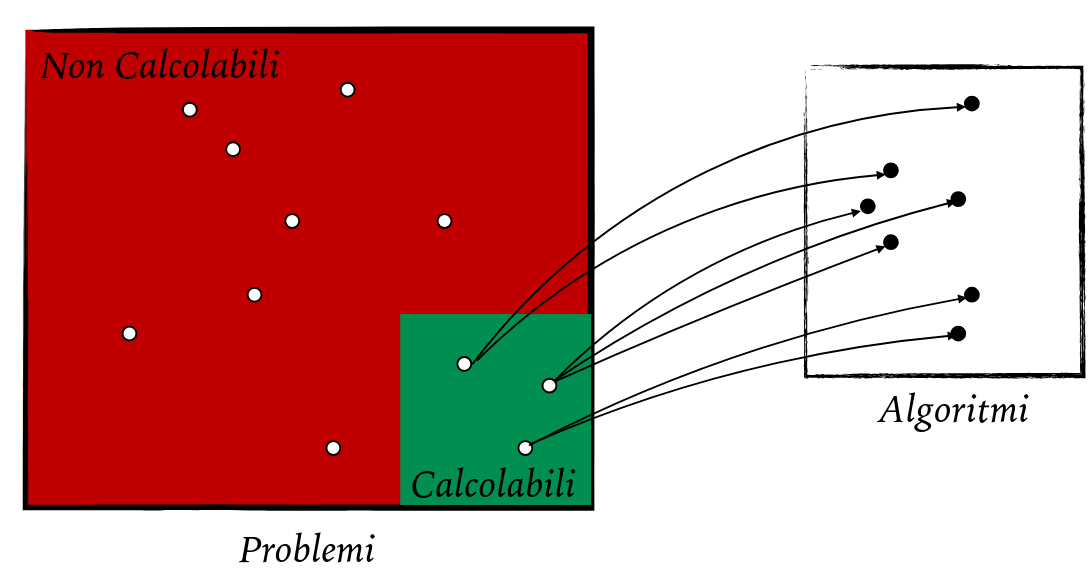
\includegraphics[width=0.8\textwidth]{cardinalita_funzioni_calcolabili}
  \caption{Cardinalità delle funzioni}
\end{figure}

\section{Principio di induzione}
Il principio di induzione è un meccanismo di definizione e dimostrazione che funziona
\textbf{solo su insiemi infiniti}. Esistono due metodi di induzione:
\begin{itemize}
  \item Induzione matematica
  \item Induzione strutturale
\end{itemize}
In questo corso tratteremo solo l'induzione matematica.

\vspace{1em}
\noindent
Un insieme \( A \) infinito con una relazione di ordine non riflessiva (senza l'uguale
perchè l'elemento non è in relazione con sè stesso): \( < \;: (A, <) \).
\( A = \mathbb{N} \) e \( < \) è l'ordinamento
stretto tra numeri naturali. La relazione di ordine deve essere \textbf{ben fondata},
quindi non devono esserci catene discendenti infinite, cioè una sequenza di elementi in
ordine decrescente infinita:
\[
  a_0 > a_1 > a_2 > a_3 > \ldots \to \text{non ben fondata}
\] 
Una relazione di ordine riflessiva non è ben fondata, perchè esistono catene
infinite:
\[
  a_0 \geq a_1 \geq a_2 \geq a_3 \geq a_3 \geq a_3 \geq \ldots \to \text{non ben fondata}
\]

\( b \) minimale in \( A : b \in A \) \( b \) è minimale se \( \forall b' < b \;.\; b' \notin A \) 
Ad esempio: \( \left\{ 1, 2, 3 \right\} \) ha come minimali (di contenimento) \( \left\{ 1, 2 \right\} \) 
e \( \left\{ 2,3 \right\} \).

\begin{definition}[Principio di induzione]
  Se \( A \) è un insisme ben fondato (con ordinamento \( < \)), e \( \Pi  \) è una
  proprietà definita sugli elementi di \( A: \Pi \subseteq A \), allora:
  \[
    \forall  a \in A \;.\; \underbrace{\Pi(a) }_{a\text{ soddisfa } \Pi} \iff
    \underbrace{
      \forall a \in A \;.\; \left[ \left[ \forall b < a \;.\; \Pi(b) \right] \Rightarrow
      \Pi(a)\right]
    }_{
      \substack{
        \text{Se dimostriamo } \Pi \text{ per ogni }\\
        \text{elemento più piccolo di } a, \\
        \text{allora } \Pi \text{ vale anche per } a
      }
    }
  \] 
  Consideriamo come caso base gli elementi minimali di \( A \):
  \[
    \text{Base}_A = \left\{ a \in A \;\left|\; a \text{ minimale}  \right.\right\}
  \] 
  Se si dimostra che \( \Pi \) vale per tutti gli elementi minimali di \( A \) (la base):
  \[
    \overbrace{
      \underbrace{
        \forall a \in \text{Base}_A \;.\; \Pi(a)
      }_{
        \substack{
          \text{Dimostriamo } \Pi \text{ per ogni }\\
          \text{elemento minimale di } A
        }
      }
    }^{\text{Base}}
    \wedge 
    \underbrace{
      \forall a \in A \setminus \text{Base}_A
    }_{
      \text{Passo induttivo}
    }
    \;.\;
    \underbrace{
      \forall b < a \;.\; \Pi(b)
    }_{
      \text{Ipotesi induttiva}
    }
    \underbrace{
      \Rightarrow \Pi(a)
    }_{
      \text{Tesi da dimostrare}
    }
  \] 
\end{definition}
\begin{example}
  Dimostriamo che:
  \[
    \forall n \in \mathbb{N} \sum_{i=1}^{n} i = \frac{n(n+1)}{2}
  \] 
  L'insieme è:
  \[
    A = \mathbb{N} \setminus \{0\} = \{1,2,3, \ldots\}
  \] 
  \begin{itemize}
    \item \textbf{Basse}
      \[
        \text{Base}_A = \{1\}
      \] 
      \begin{itemize}
        \item dimostriamo la base
          \[
            \sum_{i=1}^{1} i = n(n+1)/2 = 1(1+1)/2 = 1
          \] 
      \end{itemize}

    \item \textbf{Passo induttivo}:
      \vspace{1em}
      \noindent
      Prendo \( n \in \mathbb{N} \) 
      \begin{itemize}
        \item Ipotesi induttiva, cioè per ogni \( m < n \) vale la proprietà:
          \[
            \forall \underset{\in \mathbb{N}}{m} < n \;.\; \sum_{i=1}^{m} i =
            \frac{m(m+1)}{2}
          \] 
          Dobbiamo dimostrare la proprietà per \( n \):
          \[
            \sum_{i=1}^{n} i = \sum_{i=1}^{n-1} i + n
          \] 
          \[
            n - 1 < n \quad \text{quindi vale l'ipotesi induttiva}
          \] 
          \[
            \sum_{i=1}^{n-1} i = \frac{(n-1)(n-1+1)}{2} = \frac{(n-1)n}{2}
          \] 
          \[
            \downarrow
          \] 
          \[
            \begin{aligned}
              \sum_{i=1}^{n} i &= \sum_{i=1}^{n-1} i + n\\
                               &= \frac{(n-1)n}{2} + n\\
                               &= \frac{(n-1)n + 2n}{2}\\
                               &= \frac{n^2 - n + 2n}{2}\\
                               &= \frac{n(n+1)}{2} \quad \square
            \end{aligned}
          \] 
      \end{itemize}
  \end{itemize}
  È quindi dimostrato che:
  \[
    \forall n \in \mathbb{N} \sum_{i=1}^{n} i = \frac{n(n+1)}{2}
  \]
\end{example}

\subsection{Linguaggi formali}
\begin{definition}
  Un linguaggio formale è un insieme di stringhe costruite su un alfabeto finito \( \Sigma  \) .
\end{definition}
Solitamente un linguaggio formale \( \mathcal{L} \) è un sottoinsieme di \( \Sigma^* \),
tipicamente infiniti, ma non necessariamente:
\[
  \mathcal{L} \subseteq \Sigma^*
\] 
I linguaggi sono divisi in:
\begin{itemize}
  \item Linguaggi finiti
  \item Linguaggi regolari, il modello utilizzato è l'automa a stati finiti.
\end{itemize}
\begin{figure}[H]
  \centering
  \begin{tikzpicture}
    \draw[thick] (0,0) circle(3);
    \draw[thick] (0,1.9) circle(1);
    \node at (4,1.9) {Linguaggi formali};
    \draw[<-, thick] (0,1.9) -- (2.6,1.9);

    \node at (5,0) {Linguaggi regolari};
    \draw[<-, thick] (0,0) -- (3.6,0);
  \end{tikzpicture}
  \caption{Linguaggi formali e linguaggi regolari}
\end{figure}

\end{document}
